\chapter{  YAML to tree conversion}


The configuration information of a software app, and the data exchanged between apps,  is often stored as a  YAML data structure.

\begin{figure}[h!]
\centering
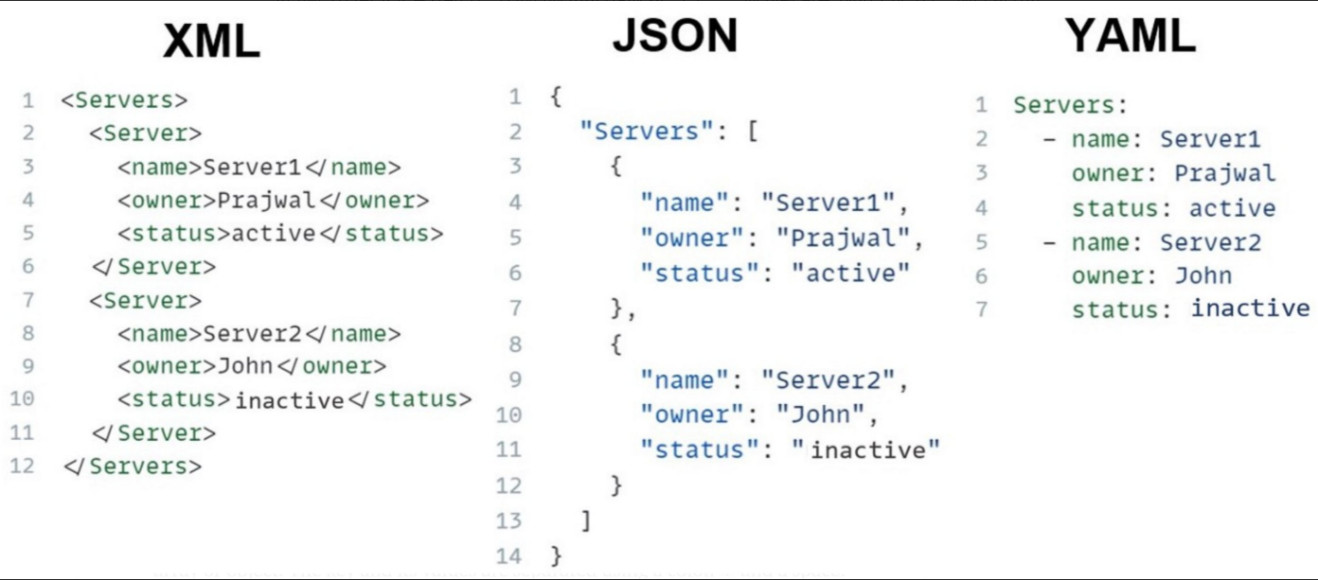
\includegraphics[width=6in]
{yaml/json-xml-yaml.jpg}
\caption{For simple data structures,
one can interconvert between JSON, XML and YAML.}
\label{fig-json-xml-yaml}
\end{figure}

YAML can be described as a human-readable data serialization language.
XML and JSON can be described that way too.
As illustrated in Fig.\ref{fig-json-xml-yaml} , for simple data structures, one can translate a data structure
from one of those languages to the others. So in this chapter, we will speak only about YAML.


In Chapter \ref{ch-dtree},
we demonstrated that a (decision) tree
can be converted without loss of
information to a bnet with the
same structure as the tree.
This is done by using marginalizer nodes.

The purpose of his chapter is not to teach
YAML to the reader.
In this chapter, we will
assume that the reader has learned YAML already,
from one of many excellent introductions to YAML
available on the internet.


The purpose of this chapter is to
demonstrate that a YAML data structure can be converted to
a tree. Then using
the results of Chapter \ref{ch-dtree}, that tree can be converted to a decision tree which can be converted to a bnet.

Like Python, YAML 
can contain 2 data structures: dictionaries
such as 

$$\boxed{\begin{array}{l}
\tt{a:1}\\
\tt{b:5}\\
\tt{c:1}
\end{array}}
\leftrightarrow
\tt{\{a:1,\quad b:5,\quad c:1\}} 
$$
and lists such as

$$
\boxed{
\begin{array}{l}
\tt{- \quad x}\\
\tt{-\quad y}\\
\tt{-\quad z}
\end{array}}
\leftrightarrow
{\tt [x,\quad y,\quad z]}
$$
In YAML, the dictionaries
have all their key-value
pairs start with the same level of indentation, and start with a letter or number.
The list items also start with
the same level of indentation, but all start with a hyphen and a space.
Lists can always be replaced by dictionaries:

$${\tt [x,\quad y,\quad z] \rarrow
\{1:x, \quad 2:y,\quad 3:z\}}
$$

$$
\boxed{
\begin{array}{l}
\tt{- \quad x}\\
\tt{-\quad y}\\
\tt{-\quad z}
\end{array}}
\rarrow
\boxed{
\begin{array}{l}
\tt{1: \quad x}\\
\tt{2: \quad y}\\
\tt{3:\quad z}
\end{array}}
$$

Once you replace in
a YAML data structure, all lists
by dictionaries,
then you have dictionaries 
with key-value pairs such that
some of the values in the pairs can lead to new dictionaries. Thus, we get a tree. See Figs.\ref{fig-yaml-list-nodes}
and Fig.\ref{fig-yaml-dict-nodes}
for examples of conversions
of YAML data structures to trees.


\begin{figure}[h!]
\centering
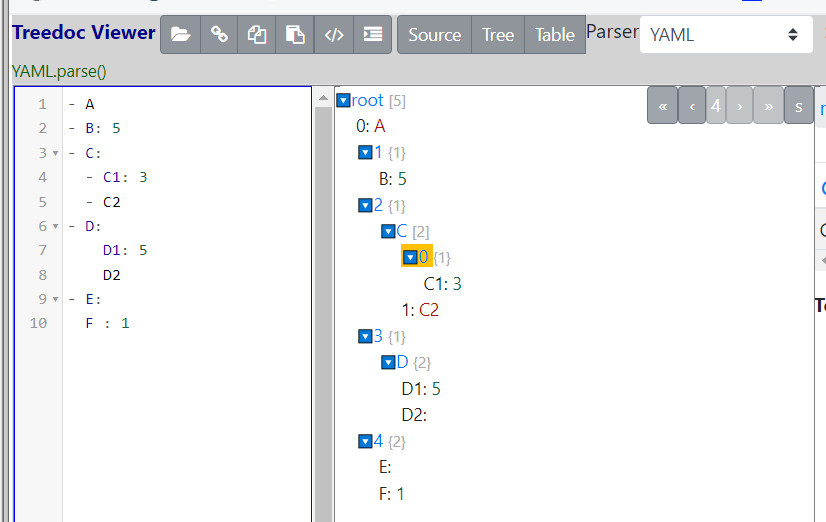
\includegraphics[width=6in]
{yaml/yaml-list-nodes.jpg}
\caption{A nodes of a YAML list can contain various cargoes.}
\label{fig-yaml-list-nodes}
\end{figure}

\begin{figure}[h!]
\centering
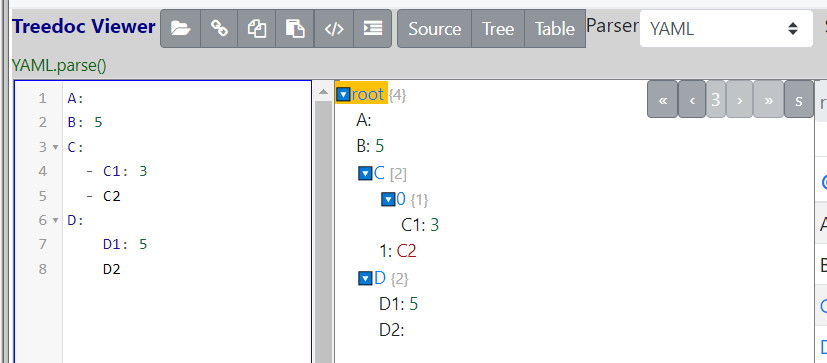
\includegraphics[width=6in]
{yaml/yaml-dict-nodes.jpg}
\caption{The nodes of a YAML dictionary can contain various cargoes. }
\label{fig-yaml-dict-nodes}
\end{figure}
